\documentclass[../main.tex]{subfiles}
\graphicspath{{\subfix{../../images/}}}

\begin{document}

A computer without an operating system is like a human without a soul. Without an OS installed on your computer, it would be no more than a fancy metal/plastic brick with silicon in it. 

\begin{figure}[H]
    \centering
    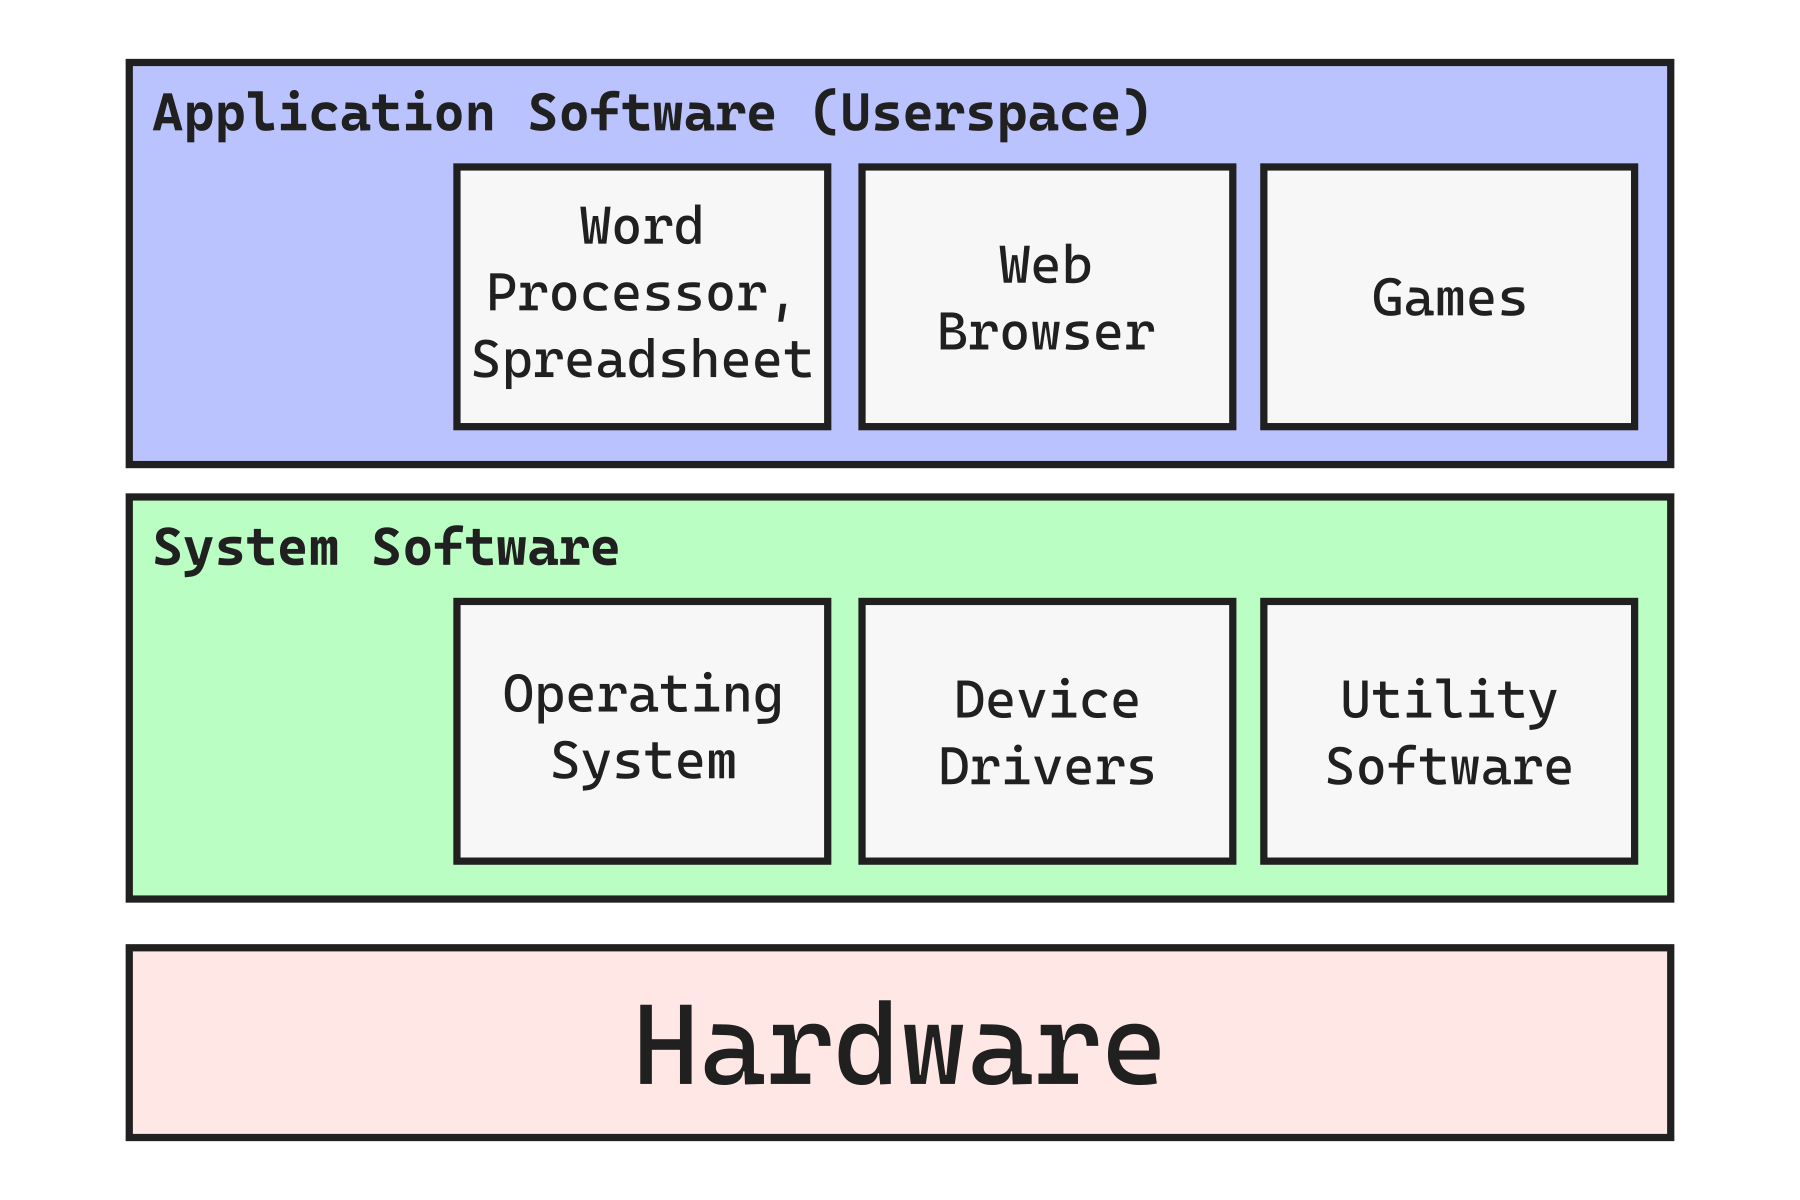
\includegraphics[width=0.85\textwidth]{software_stack.png}
    \caption{A very simplified software stack that Cambridge expects you to know.}
    \label{fig:software_stack}
\end{figure}

Figure \ref{fig:software_stack} shows the software that exists on your computer. All of this is stored in secondary storage on your boot device.

\subsection{The OS and System Software}

The operating system itself is a large set of programs that mainly run directly on the CPU, that gives the user an inteface to interact with the computer and connected devices, along with a mechanism to run programs, among others. The tasks that the OS carries out include:

\begin{enumerate}
    \item Loads device drivers for hardware and creates abstractions for application and utility software.
    \item Handles interrupts
    \item Creates and manages virtual memory (see section \ref{3:sec:virtmem}) for application and utility software
    \item Manages all files, including system files, files used by applications/programs and your files.
    \item Allows for multitasking
    \item Manages Hardware Peripherals
    \item Manages user accounts and their permissions on the computer.
    \item Provides a Human-Computer Interface (HCI)
    \item Provides Mouse/Keyboard input.
\end{enumerate}

Major Operating Systems include Microsoft Windows, Apple's macOS, Linux (GNU/Linux), and the *BSD family, among others. This is the reason why the interface you get when you use a Lenovo laptop, for example is different from if you use a Macintosh; the operating systems they use is different.

The kernel is simply a part of the operating system that creates the abstractions for hardware, so that userspace software can interact with it. On the list provided previously, items 1-5 is handled by the operating system, and the rest through special system software that is commonly grouped together with the OS. 

\subsubsection{Device Drivers}

stub

\subsubsection{Interrupts and Multitasking}

stub

\subsubsection{Virtual Memory and Memory Management}

stub

\subsubsection{File Management}

stub

\subsubsection{Hardware Peripheral Management}

stub

\subsubsection{User Accounts and Permissions}

stub

\subsubsection{Human-Computer Interfaces (HCI)}

stub

\subsection{System Software}

What sits on top of the OS includes system software. These are pieces of software that allows hardware to run correctly, provides useful functions and allows the user to communicate with the computer. There are many examples of system software:

\begin{itemize}
    \item \textbf{Compilers, Interpreters and Linkers} will be covered in section \ref{4:sec:translators_compilers_and_interpreters}, but for now, know that this is what turns your code into machine code instructions that can be used in the fetch-decode-execute cycle.
    \item \textbf{Device Drivers} are pieces of software that directly run on the CPU and is a part of the kernel; that makes peripherals like your display, mouse and keyboard function correctly. They also provide an interface so that a userspace program can use it, like drawing to the display or reading the position of the mouse.
    \item \textbf{Other Examples} include antiviruses (provides protection against malicious software), defragmentation software (compacts space on HDDs), screenshot software, screensavers, your lock screen, a file browser, file backup software, etc.
\end{itemize}

For more detailed examples of system software, refer to the textbook in the corresponding section.


\end{document}
